\documentclass{ximera}
  \outcome{Consider function values nearer and nearer to a given input value.}
  \outcome{Understand the concept of a limit.}
\begin{document}
\begin{problem}

  Consider the following graph of a function, $f$, as seen through this
  window frame.  What can we say about $f(1)$?
  \begin{image}
  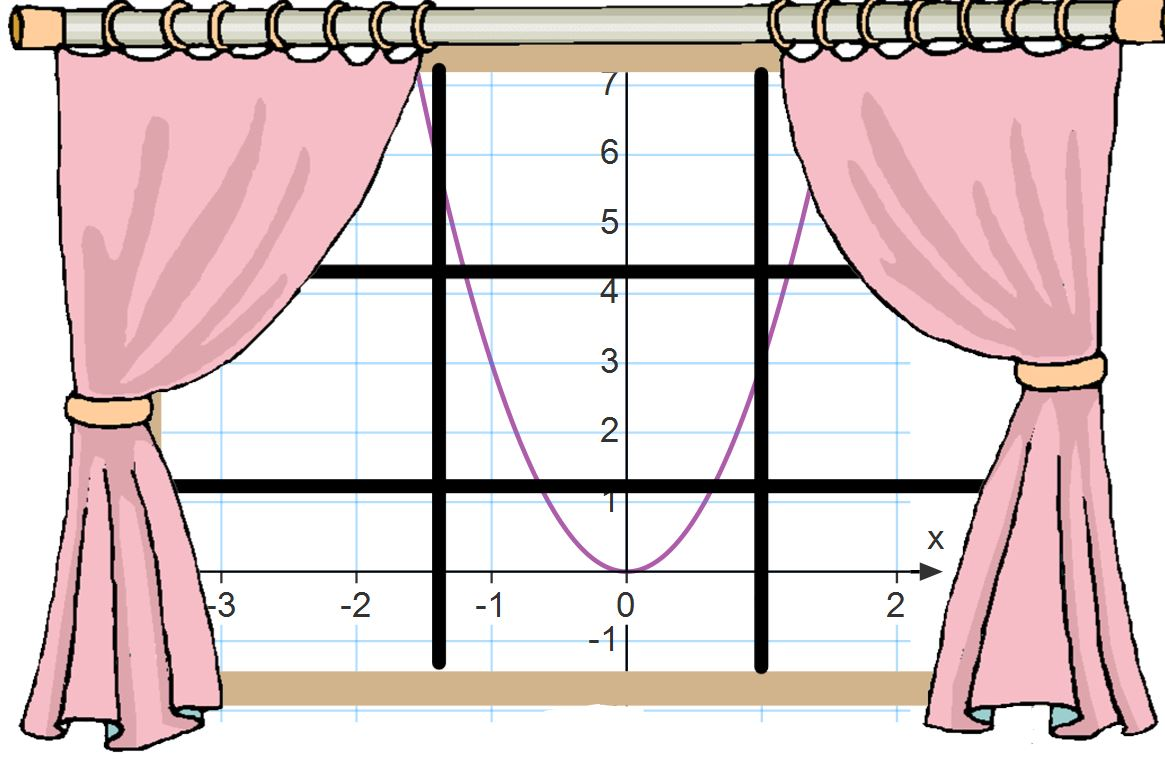
\includegraphics[scale= 0.25]{window}
  \end{image}
  \begin{multipleChoice}
    \choice{$f(1)=3$.}
    \choice{$f(1)$ is defined but we do not know it's value.}
    \choice{$f(1)$ is not defined.}
    \choice[correct]{We don't know anything about $f(1)$.}
  \end{multipleChoice}
\end{problem}
\end{document}
